
\documentclass[10pt,a4paper,twocolumn]{article}
\usepackage{times}
\usepackage{amsmath}
\usepackage{amssymb}
\usepackage{siunitx}
\usepackage{hyperref}
\usepackage{xparse}
\usepackage{relsize}
\usepackage{array}
\newcolumntype{C}[1]{>{\centering\let\newline\\\arraybackslash\hspace{0pt}}m{#1}}
\usepackage{tikz,pgfplots}
\usepgfplotslibrary{fillbetween}
\usetikzlibrary{patterns}
\pgfplotsset{compat=1.18}
\usepackage[margin=2cm]{geometry}
\usepackage[most]{tcolorbox}

\definecolor{britishracinggreen}{rgb}{0.0, 0.26, 0.15}

\tcbset{
    frame code={}
    colback=gray!70,
    colframe=white,
    boxsep=0pt,
    enlarge left by=0mm,
}
\newcommand{\capequation}[1]{\begin{tcolorbox} #1 \end{tcolorbox}\vspace{-0.5cm}}

\title{Fórmulas Física 1 - 8201 - \textbf{[Work In Progress]}}

\author{
    Guido Rodriguez\\
        \href{mailto:guerodriguez@fi.uba.ar}{\tt guerodriguez@fi.uba.ar} \\\\
    Mi perfil de github con la última versión disponible \\
        \href{https://github.com/ApophisXIV}{\tt ApophisXIV} 
}

\begin{document}
\maketitle

\section{Cinemática}

    \capequation{Arco de circunferencia}
    \begin{equation}
    s = R \cdot \theta
    \end{equation}
    
    \capequation{Velocidad Angular}
    \begin{equation}
    \vec{\Omega} = \frac{\mathrm{d} \theta}{\mathrm{d} t} \cdot \hat{k}
    \end{equation}
    
    \capequation{Aceleración Angular}
    \begin{equation}
    \vec{\gamma} = \frac{\mathrm{d} \Omega}{\mathrm{d} t} \cdot \hat{k} = \frac{\mathrm{d^2} \theta}{\mathrm{d} t^2} \cdot \hat{k}
    \end{equation}
    
    \capequation{Velocidad Tangencial-Angular (módulo)}
    \begin{equation}
    v = \Omega \cdot R
    \end{equation}
    
    \capequation{Coordenadas intrínsecas}
    \begin{center}
    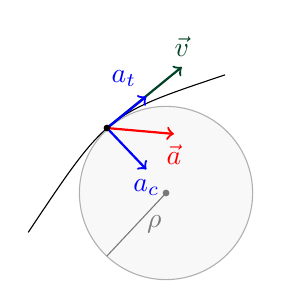
\begin{tikzpicture}
        \draw (-1.5,-1) .. controls (-0.5,0.5) .. (1,1);
        \filldraw (0.25,-0.5) circle (1pt);
        \draw (0.25,-0.5)--(-0.5,-1.3) node at (0.1,-0.9) {$\rho$};
        \filldraw[color=black!60, fill=black!5, opacity=0.5](0.25,-0.5) circle (1.1);
        \draw[->,britishracinggreen, thick] (-0.5,0.325)--(0.45,1.1) node[above]{$\vec{v}$};
        \draw[->,blue,thick] (-0.5,0.325)--(0.0,0.725) node[above left]{$a_t$};
        \draw[->,blue,thick] (-0.5,0.325)--(-0,-0.2) node[below]{$a_c$};
        \draw[->,red,thick] (-0.5,0.325)--(0.35,0.25) node[below]{$\vec{a}$};
        \filldraw (-0.5,0.325) circle (1pt);
    \end{tikzpicture}
    \end{center}
    \begin{itemize}
        \item Se descompone la aceleración en una base intrínseca ($\hat{t},\hat{n},\hat{b}$)
        \item Tomar la velocidad para construir la coordenada tangencial
        \item Si es 2D, para conseguir la coordenada $\hat{n}$ cambiar las componentes de $\hat{t}$ y cambiar el signo de alguna de ellas de tal forma que respete el sentido físico (que apunte al centro de curvatura). 
    \end{itemize}
    
    \capequation{Radio del círculo obsculador}
    \begin{equation}\label{eq:radio_circ_obs}
    \rho = \frac{||\vec{v}||^2}{a_c}
    \end{equation}
    
    \capequation{Ecuación de posición}
    \begin{equation}
        \vec{r}_{(t)}= (x_{(t)},y_{(t)},z_{(t)})
    \end{equation}
    
    \capequation{Ecuación de velocidad}
    \begin{equation}
        \vec{v}_{(t)} = \frac{\mathrm{d} \vec{r}}{\mathrm{d} t} = \left(
         \frac{\mathrm{d}x}{\mathrm{d} t},
         \frac{\mathrm{d}y}{\mathrm{d} t},
         \frac{\mathrm{d}z}{\mathrm{d} t}
        \right)
    \end{equation}
    
    \null
    \capequation{Ecuación de aceleración}
    \begin{equation}
        \vec{a}_{(t)} = \frac{\mathrm{d^2} \vec{r}}{\mathrm{d} t^2} = \left(
         \frac{\mathrm{d^2}x}{\mathrm{d} t^2},
         \frac{\mathrm{d^2}y}{\mathrm{d} t^2},
         \frac{\mathrm{d^2}z}{\mathrm{d} t^2}
        \right)
    \end{equation}
    
    \capequation{Ecuación de \textit{Jerk} (tirón)}
    \begin{equation}
        \vec{j}_{(t)} = \frac{\mathrm{d^3} \vec{r}}{\mathrm{d} t^3} = \left(
         \frac{\mathrm{d^3}x}{\mathrm{d} t^3},
         \frac{\mathrm{d^3}y}{\mathrm{d} t^3},
         \frac{\mathrm{d^3}z}{\mathrm{d} t^3}
        \right)
    \end{equation}
    
    \capequation{Movimiento relativo}
    \begin{equation}
    \begin{split}
        \vec{r}_{p/o} = \vec{r}_{p/o'} + \vec{r}_{o'/o}\\
        \vec{v}_{p/o} = \vec{v}_{p/o'} + \vec{v}_{o'/o}\\
        \vec{a}_{p/o} = \vec{a}_{p/o'} + \vec{a}_{o'/o}\\
    \end{split}
    \end{equation}
    
    \capequation{MRUV}
    \begin{equation}
    \begin{split}
        x_{(t)}&= x_{0} + v_{0} \cdot t + \frac{1}{2} \cdot a \cdot t^2\\
        {v_{f}}^2-{v_{0}}^2 &= 2 \cdot a \cdot ({x_{f}} - {x_{0}})\\
        v_{(t)}&= v_{0} + a \cdot t\\
        a_{(t)}&= cte\\
    \end{split}
    \end{equation}
    

\section{Dinámica}
    \capequation{Condición de equilibrio}
    \begin{equation}
        \Sigma\vec{F} = \vec{0}
    \end{equation}
    
    \capequation{Sistemas de referencia}
    \begin{itemize}
        \item SRI: Sistema fijo a Tierra o con velocidad constante
        \item SRNI: Sistema acelerado respecto a Tierra
    \end{itemize}
    
    \newpage
    
    \capequation{Fuerza Centrífuga (SRNI rotacional)}
    \begin{itemize}
        \item \textit{Efecto Coriolis} y \textit{Efecto Magnus}
    \end{itemize}
    \begin{equation}
        {{F_{cf}}}^* = - m \cdot \omega^2 \cdot r
    \end{equation}
    
    \capequation{Fuerza de rozamiento estática máxima}
    \begin{equation}
        F_{rs_{max}} = \mu_s \cdot N
    \end{equation}
    
    \capequation{Fuerza de rozamiento dinámica}
    \begin{equation}
        F_{rk} = \mu_k \cdot N
    \end{equation}
\section{Dinámica de fluidos}
    \capequation{Fuerza de rozamiento viscoso}
    \begin{itemize}
        \item $\mu$ (Coeficiente de viscosidad) ($\mu = 1$)
        \item k (Coeficiente de arrastre)
        \item v (El signo depende del sist. de ref. Opuesto al desplazamiento relativo)
    \end{itemize}
    \begin{equation}
        \vec{F}_{rv} = -k \cdot \vec{v}^{\ \mu}
    \end{equation}
    
    \capequation{Ley de Stokes (esferas)}
    \begin{itemize}
        \item $\mu$ (Coeficiente de viscosidad)
        \item R (Radio de la esfera)
    \end{itemize}
    \begin{equation}
        \vec{F}_{rv} = 6\pi \cdot R \cdot \mu \cdot \vec{v} 
    \end{equation}
    
    \capequation{Forma diferencial}
    \begin{equation}
        \vec{F} - \vec{F}_{rv} = m \cdot \frac{\mathrm{d}\vec{v}}{\mathrm{d}t}
    \end{equation}
    
    \capequation{Velocidad Límite}
    \begin{equation}
        v = \frac{F}{k} \left(1-e^{-\frac{k}{m}\cdot t}\right)
    \end{equation}

\section{Gravitación}
    \capequation{Fuerza de atracción gravitatoria}
    \begin{itemize}
        \item G (Constante de gravitación universal)(G = $\SI{6.673e-11}{\frac{Nm^2}{kg^2}}$)
        \item r (Distancia entre los cuerpos)
        \item Recordar \textit{Experimento de Cavendish}
    \end{itemize}
    \begin{equation}
        F_g = G \cdot \frac{m_1 \cdot m_2}{r^2}
    \end{equation}
    
\section{Masa - Resorte}
    \capequation{Ley de Hooke}
    \begin{itemize}
        \item $\Delta x$ (Deformación)
        \item -k (Constante elástica) (opuesta al desplazamiento)
        \item ${F}_{e}$ (Fuerza elástica)
    \end{itemize}
    \begin{equation}
        {F}_{e} = -k \cdot \Delta x
    \end{equation}
    
    \capequation{Velocidad de la masa en un sistema masa-resorte}
    \begin{itemize}
        \item k (Constante elástica)
        \item Si $V \in \mathbb{C}$ se entiende como un movimiento acotado
    \end{itemize}
    \begin{equation}
        |v| = \sqrt{{v_o}^2 - \frac{k}{m} \cdot (x^2 - {x_o}^2)}
    \end{equation}

    \capequation{Cota de energía en un MAS}
    \begin{equation}
        Em = A^2 \cdot \frac{k}{2}
    \end{equation}
    \begin{center}
      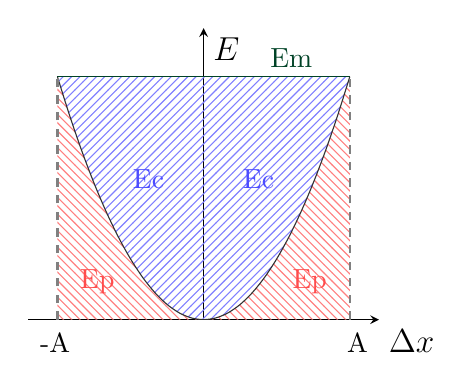
\begin{tikzpicture}[scale=0.65]
        \begin{axis}[
            ticks = none,
            axis lines = center,
            ymax=1.2,
            xmin=-1.2,
            xmax=1.2,
            xlabel = \(\Delta x\), 
            ylabel = {\(E\)}, 
            xlabel style={
                font=\large,
                at={(ticklabel cs:1)},
                anchor=north west,
            },
            ylabel style={
                font=\large,
                at={(ticklabel cs:1)},
                anchor=north west,
            },
            ]
            \addplot[smooth,britishracinggreen,name path=EM,domain=-1:1] {1} node[pos=0.8] (cotaEnergia) {};
            \node [above,color=britishracinggreen] at (cotaEnergia) {Em};
            \addplot[smooth,black!80,name path=A,domain=-1:1] {x*x};
            \addplot[draw=none,name path=B,domain=-1:1] {0};
            %
            % Filling
            \addplot[pattern=north west lines, pattern color= red!50] fill between[of=A and B,soft clip={domain=-1:1}]; % filling
            \addplot[pattern=north east lines, pattern color=blue!50] fill between[of=A and EM,soft clip={domain=-1:1}]; % filling
            %
            \addplot[thick, samples=1, dashed, black!50] coordinates {(-1,0)(-1,1)};
            \addplot[thick, samples=1, dashed, black!50] coordinates {(1,0)(1,1)};
            %
            %
        \end{axis}
        \path   (1.35,0.75) node [red!70]  {Ep}
                (5.5,0.75)  node [red!70]  {Ep}
                (2.35,2.75) node [blue!70] {Ec}
                (4.5,2.75)  node [blue!70] {Ec};
        %
        \node[text width=1cm] at (1,-0.45) {-A};
        \node[text width=1cm] at (7,-0.45) {A};
    \end{tikzpicture}
    \end{center}
    
    \capequation{Sistema masa-resorte (EDO)}
    \begin{equation}
        \frac{\mathrm{d^2x} }{\mathrm{d} t^2} + \frac{k}{m} \cdot x = 0
    \end{equation}
    Las soluciones de la ecuación son...
    \begin{equation*}
    \begin{split}
        x(t) &= A_0 \cdot \sin(\omega\cdot t + \varphi_0)\\
        v(t) &= \frac{\mathrm{dx} }{\mathrm{d} t} = \omega \cdot A_0 \cdot \cos(\omega\cdot t + \varphi_0)\\
        a(t) &= \frac{\mathrm{d^2x} }{\mathrm{d} t^2} = - \omega^2 \cdot A_0 \cdot \sin(\omega\cdot t + \varphi_0)\\
        a(t) &= \frac{\mathrm{d^2x} }{\mathrm{d} t^2} = - \omega^2 \cdot x(t)    
    \end{split}
    \end{equation*}
    
    \capequation{Período de un sistema masa-resorte}
    \begin{itemize}
        \item Pulsación o Frecuencia angulas ($\omega$)
        \item Recordar que ($\omega = 2\pi \cdot F = \frac{2\pi}{T}$)
    \end{itemize}
    \begin{equation}
    \begin{split}
        \omega &= \sqrt{\frac{k}{m}}\\
        T &= 2\pi \sqrt{\frac{m}{k}}
    \end{split}    
    \end{equation}


\section{Péndulo simple}
    \capequation{Péndulo Simple (EDO)}
    \begin{equation}
        \frac{\mathrm{d^2x} }{\mathrm{d} t^2} + \frac{g}{l} \cdot x = 0
    \end{equation}
    Las soluciones de la ecuación son...
    \begin{equation*}
    \begin{split}
        x(t) &= A_0 \cdot \sin(\omega\cdot t + \varphi_0)\\
        v(t) &= \frac{\mathrm{dx} }{\mathrm{d} t} = \omega \cdot A_0 \cdot \cos(\omega\cdot t + \varphi_0)\\
        a(t) &= \frac{\mathrm{d^2x} }{\mathrm{d} t^2} = - \omega^2 \cdot A_0 \cdot \sin(\omega\cdot t + \varphi_0)\\
        a(t) &= \frac{\mathrm{d^2x} }{\mathrm{d} t^2} = - \omega^2 \cdot x(t)    
    \end{split}
    \end{equation*}
    Las soluciones en función del ángulo...
    \begin{equation*}
    \begin{split}
        \theta_{(t)} &= \theta_0 \cdot \sin(\omega\cdot t + \varphi_0)\\
        \Omega_{(t)} &= \frac{\mathrm{d\theta} }{\mathrm{d} t} = \omega \cdot \theta_0 \cdot \cos(\omega\cdot t + \varphi_0)\\
        \gamma_{(t)} &= \frac{\mathrm{d^2\theta} }{\mathrm{d} t^2} = - \omega^2 \cdot \theta_0 \cdot \sin(\omega\cdot t + \varphi_0)\\
        \gamma_{(t)} &= \frac{\mathrm{d^2\theta} }{\mathrm{d} t^2} = - \omega^2 \cdot \theta(t)    
    \end{split}
    \end{equation*}

    \capequation{Período de un péndulo simple}
    \begin{itemize}
        \item Pulsación o Frecuencia angular ($\omega$)
        \item Recordar que ($\omega = 2\pi \cdot T = \frac{2\pi}{F}$)
        \item L (Longitud de la cuerda)
    \end{itemize}
    \begin{equation}
    \begin{split}
        \omega &= \sqrt{\frac{g}{L}}\\
        T &= 2\pi \sqrt{\frac{L}{g}}
    \end{split}    
    \end{equation}
    
    \capequation{Tensión de la cuerda}
    \begin{itemize}
        \item Recordar ecuación \ref{eq:radio_circ_obs}
    \end{itemize}
    \begin{equation}
    \begin{split}
        T &= m \cdot g \cdot cos(\theta) + m \cdot a_c\\
        T &= m \cdot g \cdot cos(\theta) + m \cdot \frac{v^2}{L}\\
        \text{Si está en reposo...}\\
        T &= m \cdot g \cdot cos(\theta)\\
    \end{split}
    \end{equation}
    

\section{Trabajo y energía}
    \capequation{Trabajo de una fuerza}
    \begin{equation}
        W_F = \int_{r_1}^{r_2} \Vec{F} \boldsymbol{\cdot} d\vec{r}
    \end{equation}
    Para una trayectoria recta...
    \begin{equation*}
        W_F = F \cdot \Delta x
    \end{equation*}

    \newpage
    
    \capequation{Potencia Media}
    \begin{equation}
        P_m = \frac{W_F}{\Delta t}
    \end{equation}
    
    \capequation{Potencia Instantánea}
    \begin{equation}
        P_i = \Vec{F} \boldsymbol{\cdot} \vec{v}_{inst}
    \end{equation}
    
    \capequation{Energía cinética (m=cte)}
    \begin{equation}
        Ec = \frac{1}{2}\cdot m \cdot v^2
    \end{equation}
    \begin{equation*}
        \Delta Ec = \frac{1}{2}\cdot m \cdot ({v_f}^2 - {v_0}^2)
    \end{equation*}
        
    \capequation{Energía potencial gravitatoria (m = cte)}
    \begin{equation}
        Epg = m \cdot g \cdot h
    \end{equation}
    \begin{equation*}
        \Delta Epg = m \cdot g \cdot (h_f - h_0)
    \end{equation*}

    \capequation{Energía potencial elástica}
    \begin{equation}
        Epe = \frac{1}{2} \cdot k \cdot x^2
    \end{equation}
    \begin{equation*}
        \Delta Epe = \frac{1}{2} \cdot k \cdot (x_f^2 - x_0^2)
    \end{equation*}
    \capequation{Teorema de las fuerzas vivas (m = cte)}
    \begin{equation}
        W_{TF} = \Delta Ec
    \end{equation}
    
    \capequation{Teorema de las fuerzas conservativas (m = cte)}
    \begin{itemize}
        \item Campos de fuerza conservativos. Una forma de intuir si un campo de fuerzas es conservativo es mediante el teorema de Schwarz. 
        \item Si es 2D... $\left( \frac{\partial f_y}{\partial x} = \frac{\partial f_x}{\partial y} \right)$
    \end{itemize}
    \begin{equation}
        W_{FC} = -\Delta Ep
    \end{equation}

    \capequation{Teorema de las fuerzas no conservativas}
    \begin{equation}
        W_{FNC} = \Delta Em
    \end{equation}
    \begin{equation*}
        \Delta Em = \Delta Ec +\Delta Ep
    \end{equation*}
    
    \capequation{EP en un campo de fuerza conservativo}
    \begin{equation}
        \vec{F} = -\left(\frac{\partial F}{\partial x} , \frac{\partial F}{\partial y} , \frac{\partial F}{\partial z} \right) = -\nabla Ep
    \end{equation}

    \newpage
    % \capequation{Diagramas energéticos}
    % \begin{equation}
    %     \begin{split}
    %         \\
    %         \\
    %         \\
    %     \end{split}
    % \end{equation}
    
    
    
\section{Sistemas de partículas}

    \capequation{Cantidad de movimiento lineal}
        \begin{equation}
            \vec{P} = m \cdot \vec{v}        
        \end{equation}
        \begin{itemize}
        \item Otros nombres posibles...
            \begin{itemize}
            \item Momento lineal
            \item Momento traslacional
            \item Cantidad de movimiento lineal
            \item Cantidad de movimiento
            \item Impetu
            \item Momentum
            \item Momento
            \end{itemize}
        \end{itemize}
        
    \capequation{Variación de la cantidad de movimiento lineal}
        \begin{equation}
            \frac{d\vec{P}}{dt} = \vec{F}
        \end{equation}

    \capequation{Fuerza media}
        \begin{equation}
            F_{med} = \frac{\Delta P}{\Delta T}
        \end{equation}
    
    \capequation{Conservación de $\vec{P}$}
        \begin{equation}
            \sum \vec{F}_{ext}=\vec{0} \rightarrow \vec{P}=cte \rightarrow \vec{v}=cte \rightarrow \vec{a}=\vec{0}
        \end{equation}
    
    \capequation{Impulso lineal}
        \begin{equation}
            \vec{I}=\int_{t_1}^{t_2} \Vec{F} \boldsymbol{\cdot} d\vec{t}
        \end{equation}
        \begin{equation}
            \vec{I} = \Delta \vec{P}        
        \end{equation}
    
    \capequation{Torque de una fuerza}
        \begin{equation}
            \overrightarrow{\tau_{\vec{F}}^{o}} = \vec{r}_o \times \vec{F}
        \end{equation}
        \begin{equation}
            \left|{\tau_{\vec{F}}^{o}}\right| = F \cdot r_o \cdot \sin{(\alpha)} = F \cdot d
        \end{equation}
        
        \begin{center}
        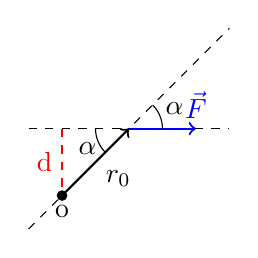
\begin{tikzpicture}[scale=0.85]
            \draw[dashed] (-1.5,0) -- (1.5,0);
            \draw[dashed] (-1.5,-1.5) -- (1.5,1.5);
            \draw[dashed,red] (-1,0) -- (-1,-1) node[anchor=east] at (-1,-0.5){d};
            \draw[thick,blue,->] (0,0) -- (1,0) node[anchor=south]{$\vec{F}$} ;
            \draw[thick,->] (-1,-1) -- (0,0) node[anchor=west] at (-0.5,-0.75){$r_0$};
            \filldraw[black] (-1,-1) circle (2pt) node[anchor=north]{o};
            \draw (0.5,0) arc (0:45:0.5) node[anchor=west] at (0.4,0.3){$\alpha$};
            \draw (-0.5,0) arc (0:45:-0.5)  node[anchor=west] at (-0.9,-0.3){$\alpha$};
        \end{tikzpicture}
        \end{center}
        \begin{itemize}
            \item \textit{d}: Brazo de palanca
            \item Otros nombres posibles (tener especial cuidado en el contexto en el que se emplean dada la similitud con los nombres alternativos de $\vec{P}$) ...
                \begin{itemize}
                    \item Fuerza rotacional
                    \item Efecto de rotación
                    \item Torca
                    \item \textit{Momento de fuerza} 
                    \item \textit{Momento}
                    \item \textit{Par motor} (específica del área mecánica)
                \end{itemize}
            \item \textbf{Fuerza Central}: Son aquellas que realizan un torque nulo respecto de un punto de referencia. (Ej: fuerzas que ``pasan'' por el punto de referencia de torques)
            \item \textbf{Cuplas}: Par de fuerzas separadas a una distancia d, de igual intensidad, misma dirección y sentidos opuestos, donde cuyo valor en módulo es $F\cdot d$. Es una herramienta útil para desacoplar el movimiento de roto-traslación de un sistema como la suma de un movimiento de traslación y uno de rotación
        \end{itemize}
        \begin{center}
            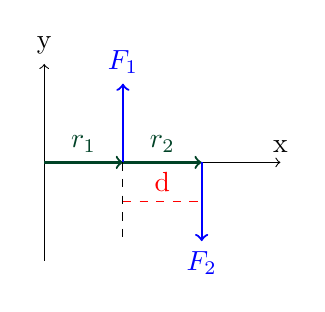
\begin{tikzpicture}
                %Axis
                \draw[->] (0,-1.25)--(0,1.25) node[above] {y};
                \draw[->] (0,0)--(3,0) node[above] {x};
                %r1 r2
                \draw[britishracinggreen,thick,->] (0,0)--(1,0) node[above] at (0.5,0) {$r_1$};
                \draw[britishracinggreen,thick,->] (1,0)--(2,0) node[above] at (1.5,0) {$r_2$};
                %Forces
                \draw[blue,thick,->] (1,0)--(1,1) node[above] {$F_1$};
                \draw[blue,thick,->] (2,0)--(2,-1) node[below] {$F_2$};
                %Distance
                \draw[red,dashed] (1,-0.5)--(2,-0.5) node[above] at (1.5,-0.5) {d};
                \draw[dashed] (1,0)--(1,-1);
            \end{tikzpicture}
        \end{center}
            
    \capequation{Cantidad de movimiento angular}
        \begin{equation}
            \vec{L}^o = \vec{r}_o \times \vec{P}_o
        \end{equation}
        \begin{equation*}
            \vec{L}^o = \vec{r}_o \times m\cdot \vec{v}
        \end{equation*}
        \begin{itemize}
            \item Otros nombres posibles (tener especial cuidado en el contexto en el que se emplean dada la similitud con los nombres alternativos de $\vec{L}$) ...
            \begin{itemize}
                \item Momento angular
                \item Momento cinético
                \item Momento rotacional
                \item Momento de momentum 
            \end{itemize}
        \end{itemize}
    
    \capequation{Variación de la cantidad de movimiento angular}
        \begin{equation}
            \frac{d\vec{L}^o}{dt} = \overrightarrow{\tau_{\vec{F}}^{o}}
        \end{equation}
    
    \capequation{Conservación de $\vec{L}^o$}
        \begin{equation}
            \sum \overrightarrow{\tau_{\vec{F}_{ext}}^{o}}=\vec{0} \rightarrow \vec{L}^o=cte \rightarrow \vec{\omega}=cte \rightarrow \vec{\gamma}=\vec{0}
        \end{equation}
        
    
            
    \capequation{Posición del centro de masa}  
        \begin{equation}
            \vec{r}_{cm} = \sum_{i=1}^{n} \frac{\vec{r}_i\cdot m_i}{M}
        \end{equation}
    
    \capequation{Velocidad del centro de masa}  
        \begin{equation}
            \vec {v}_{cm} = \sum_{i=1}^{n} \frac{\vec{v}_i\cdot m_i}{M}
        \end{equation}

    \newpage
    
    \capequation{Aceleración del centro de masa}  
        \begin{equation}
            \vec {a}_{cm} = \sum_{i=1}^{n} \frac{\vec{a}_i\cdot m_i}{M}
        \end{equation}
        
    \capequation{Cantidad de movimiento lineal del SP} 
        \begin{equation}
            \vec{P}_{sist} = \vec {P}_{cm} = {M} \cdot \vec{v}_{cm} = \sum_{i=1}^{n} \vec{v}_{i} \cdot m_i
        \end{equation}
    
    \capequation{Cantidad de movimiento angular del SP} 
        \begin{equation}
            \vec{L}_{sist}^o = \sum_{i=1}^{n} \vec{L}_{i}^o = \sum_{i=1}^n \overrightarrow{r_{i}^o} \times \overrightarrow{P_{i}^o}
        \end{equation}
        
    \capequation{Cantidad de movimiento angular (Orbital y Spin)} 
        \begin{equation}
            \begin{split}
                \vec{L}_{sist}^o &= \sum_{i=1}^{n} \vec{L}_{i}^{cm} + \overrightarrow{r}_{cm}^o \times \overrightarrow{P}_{cm}^o\\
                \vec{L}_{sist}^o &= \vec{L}_{sist}^{cm} + \vec{L}_{cm}^o\\
                \vec{L}_{sist}^o &= \vec{L}_{spin} + \vec{L}_{orbital}\\
            \end{split}
        \end{equation}
    
    \capequation{Energía potencial gravitatoria de un SP}
        \begin{equation}
            Ep = M \cdot g \cdot h_{cm}
        \end{equation}    
    
    \capequation{Energía cinética de un SP}
        \begin{equation}
            Ec_{sist}^o = \sum_{i=1}^{n} \frac{1}{2} \cdot m_i \cdot {(v_i^o)}^2
        \end{equation}
        
    \capequation{E. cinética (Orbital y Spin) - Teorema de König's} 
        \begin{equation}
        \begin{split}
            Ec_{sist}^{o} & = \frac{1}{2} \cdot M \cdot (v_{cm})^2 + \frac{1}{2} \sum_{i=1}^{n} \cdot m_i \cdot (v_i^{cm})^2\\
            Ec_{sist}^o & =  Ec_{cm}^o + Ec_{sist}^{cm}\\
            Ec_{sist}^o & = Ec_{_{orbital}} + Ec_{_{spin}}
        \end{split}
        \end{equation}
    
    \capequation{Tipos de interacciones}
        \begin{itemize}
            \item Perfectamente elástico $\rightarrow Ec^f = Ec^o \rightarrow \Delta Ec = 0$
            \item Perfectamente plástico $\rightarrow \vec{v}_{fa} = \vec{v}_{fb} $
            \item Inelástico / Endoérgico $\rightarrow Ec^f < Ec^o$
            \item Explosivo / Exoérgico $\rightarrow Ec^f > Ec^o $
        \end{itemize}
        
    \capequation{Coeficiente de restitución}
        \begin{equation}
            (\vec{v}_{2}^f-\vec{v}_{1}^f) = -e \cdot (\vec{v}_{2}^{\ o}-\vec{v}_{1}^{\ o})
        \end{equation}
        \begin{itemize}
            \item e = 1 (Perfectamente Elástico)
            \item e = 0 (Perfectamente Plástico)
            \item 0$<$e$<$1 (Inelástico / Endoérgico)
            \item e $>$ 1 (Explosivo / Exoérgico)
        \end{itemize}
\section{Cuerpo Rígido}

 \capequation{Ecuaciones de cinemática del CR}
     \begin{equation}
     \begin{split}
        \Vec{v}_p &= \Vec{v}_q + \Vec{\Omega} \times \Vec{r}_{p/q}\\
        \Vec{a}_p &= \Vec{a}_q + \Vec{\gamma} \times \Vec{r}_{p/q} + \Vec{\Omega} \times \Vec{v}_{p/q}\\
        \Vec{a}_p &= \Vec{a}_q + \Vec{\gamma} \times \Vec{r}_{p/q} + \Vec{\Omega} \times \vec{\Omega} \times \Vec{r}_{p/q}\\
     \end{split}
     \end{equation}
     \begin{itemize}
         \item Acel. de traslación: \hspace{1cm}$\overrightarrow{a_{p}^{tr}} = \Vec{a}_q$
         \item Acel. tangencial de p: \hspace{0.5cm}$\overrightarrow{a_{p/q}^{tg}} = \Vec{\gamma} \times \Vec{r}_{p/q}$
         \item Acel. centrípeta de p: \hspace{0.5cm}$\overrightarrow{a_{p/q}^{cen}} = \Vec{\Omega} \times \vec{\Omega} \times \Vec{r}_{p/q}$
     \end{itemize}
  
 \capequation{Ecuaciones de Newton del CR}
 \begin{itemize}
     \item Traslación
     \begin{equation}
         \begin{split}
            \sum F_x &= M \cdot a_{cm}^x\\
            \sum F_y &= M \cdot a_{cm}^y\\
            \sum F_z &= M \cdot a_{cm}^z\\
         \end{split}
     \end{equation}
     \item Rotación
     \begin{equation}
         \begin{split}
            \sum \tau_{x}^{cm} &= I_{x}^{cm} \cdot \gamma_{x}\\
            \sum \tau_{y}^{cm} &= I_{y}^{cm} \cdot \gamma_{y}\\
            \sum \tau_{z}^{cm} &= I_{z}^{cm} \cdot \gamma_{z}\\
         \end{split}
     \end{equation}
 \end{itemize}

 \capequation{Gráficos de velocidad/aceleración}
 
    \begin{center}
    \begin{tabular}{>{\centering\arraybackslash}m{1.5in} >{\centering\arraybackslash}m{1.5in}}
    %Traslacion pura
     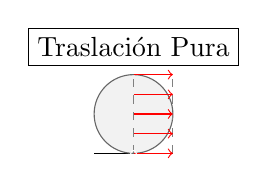
\begin{tikzpicture}
        \node[draw] at (0,1.35) {Traslación Pura};
        \draw (-0.5,0)--(0.5,0);Desliza
        \filldraw[color=black!60, fill=black!5](0,0.5) circle (0.5);
        \draw [gray,dashed] (0.5,0)--(0.5,1);
        \draw [gray,dashed] (0,0)--(0,1);
        \draw [->,red] (0,1)--(0.5,1);
        \draw [->,red] (0,0.75)--(0.5,0.75);
        \draw [->,red] (0,0.5)--(0.5,0.5);
        \draw [->,red] (0,0.25)--(0.5,0.25);
        \draw [->,red] (0,0)--(0.5,0);
        \filldraw[fill opacity=0, black!0 ] (0,0) circle (1pt);
     \end{tikzpicture}
    &
    %Rotacion pura
     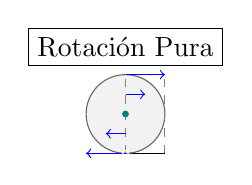
\begin{tikzpicture}
        \node[draw] at (0,1.35) {Rotación Pura};
        \draw (-0.5,0)--(0.5,0);
        \filldraw[color=black!60, fill=black!5](0,0.5) circle (0.5);
        \draw [gray,dashed] (0.5,0)--(0.5,1);
        \draw [gray,dashed] (0,0)--(0,1);
        \draw [->,blue] (0,1)--(0.5,1);
        \draw [->,blue] (0,0.75)--(0.25,0.75);
        \filldraw[teal] (0,0.5) circle (1pt);
        \draw [->,blue] (0,0.25)--(-0.25,0.25);
        \draw [->,blue] (0,0)--(-0.5,0);
        \filldraw[fill opacity=0, black!0 ] (0,0) circle (1pt);
     \end{tikzpicture}
    \\
    %Rototraslacion perfecta
     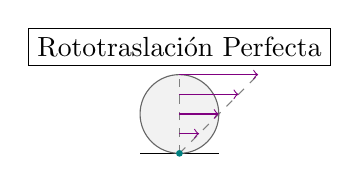
\begin{tikzpicture}
        \draw (-0.5,0)--(0.5,0);
        \filldraw[color=black!60, fill=black!5](0,0.5) circle (0.5);
        \draw [gray,dashed] (0,0)--(1,1);
        \draw [gray,dashed] (0,0)--(0,1);
        \draw [->,violet] (0,1)--(1,1);
        \draw [->,violet] (0,0.75)--(0.75,0.75);
        \draw [->,violet] (0,0.5)--(0.5,0.5);
        \draw [->,violet] (0,0.25)--(0.25,0.25);
        \filldraw[teal] (0,0) circle (1pt);
        \node[draw] at (0,1.35) {Rototraslación Perfecta};
     \end{tikzpicture}
    &
    \vspace{0.5cm}
    %Rototraslacion imperfecta
     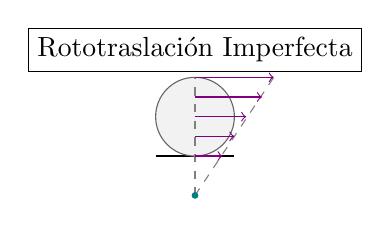
\begin{tikzpicture}
        \node[draw] at (0,1.35) {Rototraslación Imperfecta};
        \draw (-0.5,0)--(0.5,0);
        \filldraw[color=black!60, fill=black!5](0,0.5) circle (0.5);
        \draw [gray,dashed] (0,-0.5)--(1,1);
        \draw [gray,dashed] (0,-0.5)--(0,1);
        \draw [->,violet] (0,1)--(1,1);
        \draw [->,violet] (0,0.75)--(0.85,0.75);
        \draw [->,violet] (0,0.5)--(0.65,0.5);
        \draw [->,violet] (0,0.25)--(0.5,0.25);
        \draw [->,violet] (0,0)--(0.35,0);
        \filldraw[teal] (0,-0.5) circle (1pt);
     \end{tikzpicture}
    \end{tabular}
    \end{center}
    
 \capequation{Centro Instantáneo de Rotación}
    \begin{itemize}
        \item Por definición $v_{cir} := 0_{m/s}$
        \item El CIR coincide con el punto de contacto del cuerpo con la superficie si este se encuentra en un estado de rotación perfecta o bajo condición de rotación sin desplazamiento relativo entre él y la superficie (\textit{RSD})
        \item Útil para ciertos planteos de torques cuando la fuerza que lo realiza es desconocida.
    \end{itemize}
\newpage

 \capequation{Momento de inercia}
 \begin{equation}
        I^{A} = \sum_{i=1}^{\infty} m_i \cdot d^2
 \end{equation}
 \begin{itemize}
    \item Generalización...
    \begin{equation*}
        I^{A} = \int_V \delta \cdot \xi^2 \,dV
    \end{equation*}
    \item En función de $L$...
    \begin{equation}
        I^{A} =\frac{L^A}{\Omega}
    \end{equation}
 \end{itemize}

\capequation{Momentos de inercia notables}
\begin{center}
\begin{tabular}{>{\centering\arraybackslash}m{1.25in} >{\centering\arraybackslash}m{1.25in}}
    Cilindro macizo $I^{cm} = \frac{1}{2} \cdot M \cdot   R ^ 2       $&
    Cilindro hueco  $I^{cm} = \frac{1}{2} \cdot M \cdot  (R ^ 2 + r^2)$
    \\\\
    Esfera maciza $I^{cm} = \frac{2}{5} \cdot M \cdot R ^ 2$&
    Esfera hueca  $I^{cm} = \frac{2}{3} \cdot M \cdot  (R^ 2 + r^2)$
    \\\\
    Barra delgada $I^{cm} = \frac{1}{12} \cdot M \cdot L ^ 2$&
    Aro delgado  $I^{cm} = M \cdot  (R^ 2 + r^2)$
    \\\\
    Partícula $I^{cm} = m \cdot d ^ 2$&
\end{tabular}
\end{center}
 
 \capequation{Teorema de Steiner}
 \begin{equation}
     I^A = I^{cm} + M\cdot d^2
 \end{equation}
 
\capequation{Energía potencial de un CR}
\begin{itemize}
    \item Por ser un CR su Ep es únicamente gravitatoria, si hubiera elástica sería un \textit{soft-body}, es decir, presenta deformaciones.
    \item El CR por ser un tipo de SP, la energía potencial gravitatoria será igual a la mencionada anteriormente
    \begin{equation}
        Ep = M \cdot g \cdot h_{cm}
    \end{equation}    
\end{itemize}

\capequation{Energía cinética de un CR}
\begin{equation}
\begin{split}
    Ec_{_{CR}}^{o} & = \frac{1}{2} \cdot M \cdot v_{cm}^2 + \frac{1}{2} I^{cm} \cdot \Omega^2\\
    Ec_{_{CR}}^o & = Ec_{_{orbital}} + Ec_{_{spin}}\\
    Ec_{_{CR}}^o & = Ec_{_{traslacional}} + Ec_{_{rotacional}}\\
\end{split}
\end{equation}
\begin{itemize}
    \item Si lo analizamos desde el CIR la EC total será la de rotación. Útil para conocer la incógnita de EC total (Recordar aplicar Steiner para 
    conseguir $I^{cir}$)
    \begin{equation}
        Ec_{_{CR}}^{cir} = \frac{1}{2} \cdot I^{cir} \cdot \Omega^2
    \end{equation}
\end{itemize}

\capequation{Energía mecánica de un CR}
\begin{equation}
    Em = M \cdot g \cdot h_{cm} + \frac{1}{2} \cdot M \cdot v_{cm}^2 + \frac{1}{2} I^{cm} \cdot \Omega^2
\end{equation}

\capequation{Trabajo del torque}
\begin{equation}
    W_{\Vec{\tau}_{\vec{F}}^{\ o}} = \int_{\theta_1}^{\theta_2} \Vec{\tau}_{\vec{F}}^{\ o}  \boldsymbol{\cdot} \,d\vec{\theta}
\end{equation}

\capequation{Trabajo de la fuerza de rozamiento}
\begin{itemize}
    \item Si el cuerpo rueda sin deslizar, el trabajo que realiza la fuerza de rozamiento es nulo pues no hay desplazamiento relativo entre la superficie con rozamiento y el cuerpo en cuestión.
    \item Caso contrario, se deberá conocer ``cuanto patina'' para estimar el trabajo de la fuerza de rozamiento.
\end{itemize}

\capequation{Cantidad de movimiento angular del CR}
\begin{equation}
\begin{split}
    \vec{L}^{sist} = \vec{L}^{spin} + \vec{L}^{orbital}\\
    \vec{L}^{sist} = I^{cm} \cdot \Vec{\Omega} + M \cdot \Vec{v}_{cm}
\end{split}
\end{equation}

\begin{equation}
    \vec{L}^{cm} = I^{cm} \cdot \Vec{\Omega}
\end{equation}

\begin{equation}
    \vec{L}^{cir} = I^{cir} \cdot \Vec{\Omega}
\end{equation}


\capequation{Péndulo físico (EDO)}
\begin{equation}
    \frac{d^2 \theta}{dt} + \frac{M\cdot g\cdot d}{I^o} \cdot \sin{\theta} = 0
\end{equation}
\begin{itemize}
    \item Si consideramos ángulos pequeños podemos encontrar la siguiente relación...
    \begin{equation}
        \omega^2 = \frac{M\cdot g\cdot d}{I^o}
    \end{equation}
\end{itemize}

\capequation{Período de un péndulo físico}
\begin{equation}
    T = 2\pi\sqrt{\frac{I^{cm}+M\cdot d^2}{M\cdot g\cdot d}}
\end{equation}

\capequation{Péndulo sincrónico}
\begin{itemize}
    \item Se busca equiparar el período de oscilación de un péndulo físico con uno simple (herramienta útil para medir momentos de inercia).
    \item Se busca la longitud l del péndulo simple que provoque que su período de oscilación sea el mismo que el del CR.
    \item k (Radio de giro baricéntrico) ($k^2 \cdot M = I^{cm}$)
    \item l (Longitud reducida)
    \item d (Distancia del punto propio del CR al centro de rotación)
    \begin{equation}
        l = \frac{k^2}{d} + d
    \end{equation}
\end{itemize}
\section{Hidrodinámica}
\capequation{Magnitudes básicas}
\begin{itemize}
    \item Densidad $\rho=\frac{m}{V}$ 
    \item Peso específico $\Vec{\gamma} = \rho \cdot \Vec{g}$
    \item Densidad relativa $\rho_{rel}=\frac{\rho}{\rho_{H_2O}}$ 
    \item Presión $P = \frac{F}{A} \left[\frac{N}{m^2}\right]$ $[Pa]$
\end{itemize}

\capequation{Presión}
\begin{itemize}
    \item $P_{atm}$ (Presión atmosférica)
    \item $P_{m}$ (Presión manométrica)
    \item Presión absoluta
    \begin{equation}
        P_T = P_{atm} + P_m
    \end{equation}
    \item Forma general
    \begin{equation}
        P_1 = P_2 + \rho g h
    \end{equation}
\end{itemize}

\capequation{Ley de Pascal}
\begin{itemize}
    \item $A_i$ (Área donde es aplicada la fuerza)
    \item $F_i$ (Fuerza aplicada sobre el área asociada)
    \item Útil para prensas hidráulicas
    \begin{equation}
        \frac{F_1}{A_1} = \frac{F_2}{A_2}
    \end{equation}
    \item Factor multiplicador de fuerza
    \begin{equation*}
        F_2 = F_1 \cdot \frac{A_2}{A_1}
    \end{equation*}
\end{itemize}

\capequation{Ecuación de continuidad}
\begin{equation}
    v_1 \cdot S_1 = v_2 \cdot S_2
\end{equation}

\capequation{Bernoulli}
\begin{equation}
    \frac{P}{\rho g} + y + \frac{v^2}{2g} = cte
\end{equation}
\begin{equation}
    P_1 + \frac{1}{2}\rho {v_1}^2 + \rho g h = cte
\end{equation}

\newpage

\section{Óptica geométrica}
\capequation{Índice de refracción}
\begin{itemize}
    \item Absoluto
    \begin{equation}
        n = \frac{c_o}{v_p}
    \end{equation}
    \item Relativo
    \begin{equation}
        n = \frac{n_1}{n_0}
    \end{equation}
\end{itemize}

\capequation{Ley de Snell}
\begin{equation}
    n_1 \sin{\theta_1} = n_2 \sin{\theta_2}
\end{equation}

\capequation{Corrimiento lateral en láminas de caras paralelas}
\begin{itemize}
    \item h (Espesor de la placa)
    \item d (Desviación)
    \item $\theta_i$ (Ángulo incidente Snell)
    \item $\theta_r (\beta)$ (Ángulo reflejado Snell)
\end{itemize}
\begin{equation}
    d = \frac{\sin{(\theta_i - \theta_r)} \cdot h}{\cos{(\theta_r)}}
\end{equation}
\begin{figure}[h]
    \centering
    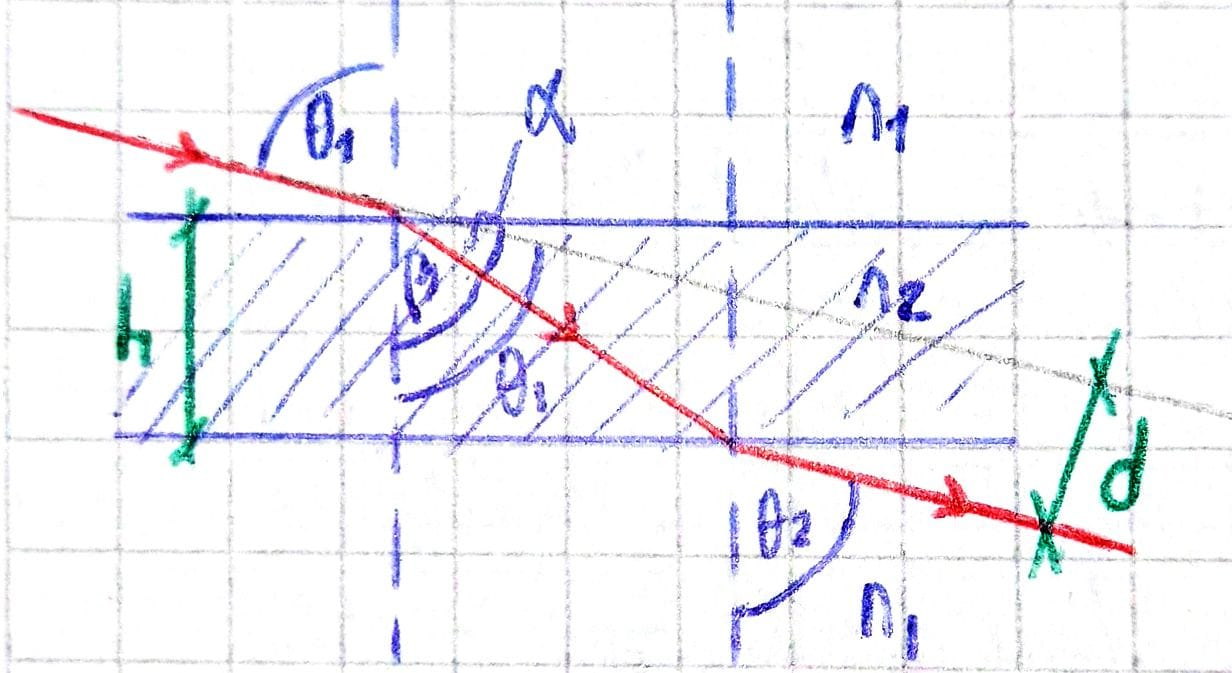
\includegraphics[scale=0.12]{images/laminas_paralelas.png}
\end{figure}

\capequation{Longitud óptica}
\begin{itemize}
    \item n (Índice de refracción)
    \item S (Espesor de la superficie)
\end{itemize}
\begin{equation}
    L_{opt} = n_i \cdot S_i
\end{equation}

\capequation{Fórmula de Descartes para espejos esféricos}
\begin{itemize}
    \item X (Posición del objeto)
    \item X' (Posición de la imagen)
    \item F (Foco del espejo)
    \item R (Radio de curvatura del espejo)
    \begin{equation}
        \frac{1}{X} + \frac{1}{X'} = \frac{1}{F} + \frac{2}{R} 
    \end{equation}
    \item El foco en un es espejo es único y es
    \begin{equation*}
        f = \frac{R}{2}
    \end{equation*}
    \begin{equation*}
        f' = \frac{R}{2}
    \end{equation*}
\end{itemize}

\capequation{Aumentos en espejos}
\begin{equation}
    A = \frac{X'}{X} = -\frac{Y'}{Y}
\end{equation}

\capequation{Dioptras esféricas}
\begin{itemize}
    \item Ecuación general
    \begin{equation}
        \frac{n_2}{X'} - \frac{n_1}{X} = \frac{(n_2 - n_1)}{R}
    \end{equation}
    \item Foco objeto
    \begin{equation}
        f = -\frac{n_1 \cdot R}{n_2 - n_1}
    \end{equation}
    \item Foco imagen
    \begin{equation}
        f = \frac{n_2 \cdot R}{n_2 - n_1}
    \end{equation}
    \item Relación de focos
    \begin{equation}
        \frac{f}{f'} = -\frac{n_1}{n_2}
    \end{equation}
    \item Notar que si la dioptra es plana el $R\rightarrow \infty$ por lo que queda
    \begin{equation*}
        X' = X \cdot \frac{n_2}{n_1}
    \end{equation*}
    \item La dioptra puede ser convergente o divergente
\end{itemize}

\capequation{Aumentos en dioptras}
\begin{itemize}
    \item Planas $A = +1$ (Aumento unitario. Imagen derecha)
    \item Esféricas
    \begin{equation}
        A = \frac{n_1 \cdot X'}{n_2 \cdot X} = \frac{Y'}{Y}
    \end{equation}
\end{itemize}

\capequation{Lentes}
\begin{itemize}
    \item Las lentes pueden ser convergentes o divergentes y a su vez (geométricamente):
    \begin{itemize}
        \item Bi-convexa
        \item Bi-concava
        \item Plano - Convexa
        \item Plano - Concava
        \item Concava - Convexa (meñisco)
    \end{itemize}
    \item Fórmula general
    \begin{itemize}
        \item $n_l$ (Índice de refracción de la lente)
        \item $n_m$ (Índice de refracción del medio)
    \end{itemize}
    \begin{equation}
        \frac{1}{X} - \frac{1}{X'} = \frac{n_m - n_l}{n_l} \cdot \left( \frac{1}{R_2} - \frac{1}{R_1}\right)
    \end{equation}
    \item Foco Objeto
    \begin{equation}
       \frac{1}{F} = \frac{n_m - n_l}{n_l} \cdot \left( \frac{1}{R_2} - \frac{1}{R_1}\right)
    \end{equation}
    \item Foco Imagen
    \begin{equation}
       -\frac{1}{F'} = \frac{n_m - n_l}{n_l} \cdot \left( \frac{1}{R_2} - \frac{1}{R_1}\right)
    \end{equation}
    \item Si los focos son virtuales (divergente), si son reales (convergentes)
\end{itemize}

\capequation{Aumentos en lentes}
\begin{equation}
    A = \frac{X'}{X} = \frac{Y'}{Y}
\end{equation}

\capequation{Potencia de una lente}
\begin{itemize}
    \item Se mide en \textit{dioptrías} $\left[\frac{1}{m}\right]$
    \begin{equation}
        P = \frac{1}{F} = \frac{n_m - n_l}{n_l} \cdot \left( \frac{1}{R_2} - \frac{1}{R_1}\right)
    \end{equation}
\end{itemize}

\capequation{Prismas}
\begin{figure}[h]
    \centering
    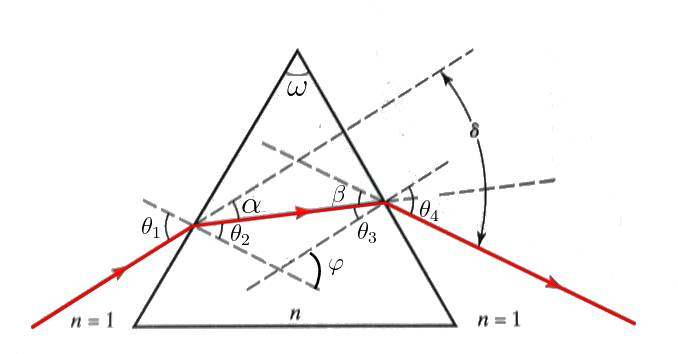
\includegraphics[scale=0.3]{images/prisma.jpg}
\end{figure}
\begin{itemize}
    \item El ángulo A de la imagen lo llamaré $\omega$
    
    \item Para ángulos pequeños la desviación mínima será
    \begin{equation}
        \delta_{min} = (n-1) \omega
    \end{equation}
    \item Para conocer el índice del prisma
    \begin{equation}
        n = \frac{\sin(\frac{\delta_{min} + \omega}{2})}{\sin(\frac{\omega}{2})}
    \end{equation}
    \item Ángulos notables
        \begin{align*}
            \alpha    &= \theta_1 - \theta_2  & \beta  &= \theta_4 - \theta_3 \\
            \theta_2  &= \frac{\omega}{2}     & \delta &= \theta_1 + \theta_4 - \omega \\
        \end{align*}
        ($2\theta_1$ es porque $\theta_1 = \theta_4$)
        \begin{equation*}
            \delta_{min} = 2\theta_1 - \omega
        \end{equation*}
\end{itemize}
\newpage
\section{Óptica Física}
\capequation{Interferencia - Experiencia de Young}
\begin{itemize}
    \item Fenómeno de interferencia absoluta
    \item En una pantalla lejana (frente de ondas planos) a las rendijas (las cuales a su vez se comportan como fuentes por el principio de Huygens) se observa un patrón de interferencia provocado por una o más fuentes \textbf{coherentes}.
    \item \textbf{Fuentes coherente}: Fuente monocromática, diferencia de fase constante
    \item Máximos
    \begin{equation}
        x^{max} = n \cdot \frac{\lambda D}{d} , n \in \mathbb Z
    \end{equation}
    \item Mínimos (N: Número de fuentes)
    \begin{equation}
        x^{min} = \frac{n}{N} \cdot \frac{\lambda D}{d} , n \in \mathbb Z \quad \land \quad n \neq N
    \end{equation}
    \item Otra forma de calcular los máximos y mínimos en función del ángulo $\theta$x
    \begin{equation}
    \begin{split}
       d \sin(\theta^{max}) &= n \lambda \\
       d \sin(\theta^{min}) &= \frac{2n + 1}{2} \lambda 
    \end{split}
    \end{equation}
    \item Cantidad de máximos principales y secundarios
    \begin{itemize}
        \item Principales:
        \begin{equation}
            N^o_{ppal} = N - 1
        \end{equation}
        \item Secundarios:
        \begin{equation}
            N^o_{sec} = N - 2
        \end{equation}
    \end{itemize}
    \item Intensidad Máxima (ángulos pequeños) (N: Número de fuentes)
    \begin{equation}
        I = N^2 \cdot I_0
    \end{equation}
\end{itemize}

\capequation{Difracción}
\begin{itemize}
    \item Mínimos de difracción (\textbf{b}: ancho de rendija. Similar al parámetro d en interferencia)
    \begin{equation}
        x^{min} = n \cdot \frac{\lambda D}{b} , n \in \mathbb Z^*
    \end{equation}
    \item Mínimos de difracción en función del ángulo
    \begin{equation}
        b \sin(\theta^{min}) = n \lambda , n \in \mathbb Z^*
    \end{equation}
\end{itemize}

\capequation{Redes de difracción}
\begin{itemize}
    \item Constante de la red (\textbf{d}: separación de ranuras. No confundir con ancho de ranuras \textbf{b})
    \begin{equation}
        C = \frac{1}{d}
    \end{equation}
    \item Máximo orden observable
    \begin{equation}
        n_{max} = \frac{d}{\lambda}
    \end{equation}
\end{itemize}
\section{Ondas}
\capequation{Ondas mecánicas}
\begin{itemize}
    \item Propagación de energía en el medio material, no así de materia.
    \item Pueden ser de propagación transversal, longitudinal o una combinación de ambas
    \begin{itemize}
        \item \textbf{Transversal}: Perturbación perpendicular a la dirección de propagación
        \item \textbf{Longitudinal}: Perturbación paralela a la dirección de propagación
    \end{itemize}
    \item Sentido de propagación
    \begin{itemize}
        \item Viajeras
        \item Reflejadas
        \item Estacionarias
    \end{itemize}
\end{itemize}

\capequation{Ecuación de una onda viajera}
\begin{itemize}
    \item El signo depende del sentido de propagación. Negativo izquierda a derecha, positivo caso contrario.
    \begin{equation}
        \psi_{(x,t)} = A \sin(kx \pm \omega t + \phi)
    \end{equation}
\end{itemize}

\capequation{Elementos de la onda}
\begin{align}
    f &= \frac{1}{T}            & f&=\frac{v_p}{\lambda} & T &=\frac{1}{f}\\
    v_p &= f \cdot \lambda & v_p &= \frac{\lambda}{T} &\\
    \omega &=2\pi \cdot f & \omega &= \frac{2\pi}{T}   & \omega&= k \cdot v_p \\
    k &= \frac{2\pi}{\lambda}   & k&= \frac{\omega}{v_p} & 
\end{align}

\capequation{Velocidad, posición y aceleración de perturbación}
\begin{equation}
\begin{split}
    r_{(x,t)} &= \ \ \ A \sin(kx \pm \omega t + \phi_0)\\
    v_{(x,t)} &= \ \ \ A \cos(kx \pm \omega t + \phi_0)(\pm\omega)\\
    a_{(x,t)} &= -A \sin(kx \pm \omega t + \phi_0)(\pm\omega)^2\\
\end{split}
\end{equation}

\capequation{Velocidad de propagación en diferentes medios}
\vspace{0.25cm}
\begin{itemize}
    \item Todas son expresadas en $[\frac{m}{s}]$
    \item Cuerda (siempre transversales)
    \begin{equation}
        v_p=\sqrt{\frac{T}{\mu}}
    \end{equation}
    \item Varilla
        \begin{itemize}
            \item Transversales
            \item G: Modulo de Young transversal
            \begin{equation}
                v_p=\sqrt{\frac{G}{\rho}}
            \end{equation}
            \item Longitudinales
            \item Y: Modulo de Young longitudinal
            \begin{equation}
                v_p=\sqrt{\frac{Y}{\rho}}
            \end{equation}
        \end{itemize}
    \item Gases
    \begin{itemize}
        \item General
        \begin{equation}
            v_p = \sqrt{\frac{B}{\rho}}
        \end{equation}
        \item En función de la temperatura del aire
        \begin{equation}
            v_p = 330\sqrt{1+\frac{\Delta t}{273C^o}} 
        \end{equation}
    \end{itemize}
    \item Resortes
    \begin{equation}
        v_p = \sqrt{\frac{k\cdot L}{\mu}}
    \end{equation}
\end{itemize}

\capequation{Ondas en un gas}
\begin{itemize}
    \item Onda de desplazamiento
    \begin{equation}
        \psi_{(x,t)} = P_0 \sin(kx \pm \omega t + \phi_0)
    \end{equation}
    \item Onda de presión
    \begin{equation}
        P_{(x,t)} = P_0 \cos(kx \pm \omega t + \phi_0)
    \end{equation}
\end{itemize}

\capequation{Intensidad de una onda}
\vspace{0.25cm}
\begin{itemize}
    \item A: Amplitud
    \item $\rho$: Densidad volumétrica
    \item $\omega$: Pulsación
    \item $v_p$: Velocidad de propagación del medio
\end{itemize}
\begin{equation}
    I = \frac{1}{2} \cdot A^2 \cdot \rho \cdot v_p \cdot \omega^2
\end{equation}

\capequation{Intensidad de una onda de presión sonora (Aire)}
\vspace{0.25cm}
\begin{itemize}
    \item P: Presión
    \item $\rho$: Densidad volumétrica
    \item $\omega$: Pulsación
    \item $v_p$: Velocidad de propagación del medio
\end{itemize}
\begin{equation}
    I = \frac{P^2}{2\cdot \rho \cdot v_p}
\end{equation}

\capequation{Potencia de una onda}
\begin{itemize}
    \item Notar que difiere en $\mu$ con la ecuación de Intensidad
    \item A: Amplitud
    \item $\rho$: Densidad lineal
    \item $\omega$: Pulsación
    \item $v_p$: Velocidad de propagación del medio
\end{itemize}
\begin{equation}
    P = \frac{1}{2} \cdot A^2 \cdot \mu \cdot v_p \cdot \omega^2
\end{equation}

\capequation{Potencia (expresión equivalente)}
\begin{itemize}
    \item $I$: Intensidad
    \item $s$: Sección
\end{itemize}
\begin{equation}
    P = I \cdot s
\end{equation}

\capequation{Energía media}
\begin{equation}
    E = P \cdot \Delta t
\end{equation}
\begin{equation}
    E = \frac{1}{2} \cdot A^2 \cdot \mu \cdot v_p \cdot \omega^2
\end{equation}

\capequation{Densidad de Energía}
\begin{itemize}
    \item Notar que difiere en $v_p$ con la ecuación de Intensidad
\end{itemize}
\begin{equation}
    E = \frac{1}{2} \cdot A^2 \cdot \rho \cdot \omega^2
\end{equation}

\capequation{Decibeles}
\vspace{0.25cm}
\begin{itemize}
    \item N.I.S. (Nivel de Intensidad Sonora)
    \item Mínimo nivel de intensidad sonora audible: \\ $I_0 = 10^{-12} \left[\frac{W}{m^2}\right]$
\end{itemize}
\begin{equation}
    \beta = 10\log\left(\frac{I}{10^{-12}}\right)
\end{equation}

\capequation{Efecto Doppler}
\begin{itemize}
    \item $v_p$: Velocidad de propagación Tratarlo con sentido (signo).
    \item $v_o$: Velocidad de observador Tratarlo con sentido (signo).
    \item $v_f$: Velocidad de fuente
    \item $f$: Frecuencia emitida
    \item $f'$: Frecuencia percibida
\end{itemize}
\begin{equation}
    f' = f \left(\frac{v_p - (v_o)}{v_p - (v_f)}\right)
\end{equation}

\capequation{Ecuación de superposición de ondas}\vspace{0.25cm}
\begin{itemize}
    \item Identidades trigonométricas
    \begin{equation*}
        \begin{split}
            \sin(A) + \sin(B) &= 2 \sin\left(\frac{A+B}{2}\right)\cos\left(\frac{A-B}{2}\right)\\
            \cos(A) + \cos(B) &= 2 \cos\left(\frac{A+B}{2}\right)\cos\left(\frac{A-B}{2}\right)\\
        \end{split}
    \end{equation*}
    
    \item Superposición general 
    \begin{equation}
    \begin{split}
        \psi_{(x,t)} &= 2A \cdot \sin\left(kx + {\frac{\phi_1 +\phi_2}{2}}\right) \cdot \cos\left({\omega t+ \frac{\phi_1 - \phi_2}{2}}\right)\\
        \psi_{(x,t)} &= 2A \cdot \cos\left(kx + {\frac{\phi_1 +\phi_2}{2}}\right) \cdot \cos\left({\omega t+ \frac{\phi_1 - \phi_2}{2}}\right)\\
    \end{split}
    \end{equation}
    
    \item Superposición totalmente constructiva
    \begin{equation}
        \psi_{(x,t)} = 2A \cdot \cos\left({kx-\omega t}\right)
    \end{equation}
    
    \item Superposición totalmente destructiva
    \begin{equation}
        \psi_{(x,t)} = 0
    \end{equation}
\end{itemize}

\capequation{Tubo Abierto-Abierto}
\begin{align}
    f_n &= n \cdot \frac{V_p}{2L}   &  f_n &= n \cdot f_0 \\
    \lambda&=\frac{2L}{n}           &  L   &= \frac{n\cdot\lambda}{2}
\end{align}

\capequation{Tubo Abierto-Cerrado}
\begin{align}
    f_n &= (2n+1) \cdot \frac{V_p}{4L}  &  f_n &= (2n+1) \cdot f_0 \\ 
    \lambda&=\frac{4L}{(2n+1)}          &  L   &= \frac{(2n+1)\cdot\lambda}{4}
\end{align}

\end{document}
